\documentclass[a4paper]{article}
\usepackage{a4wide}
\usepackage{Sweave}
\newcommand\code\texttt
\newcommand\R{\textsf{R}}
\newcommand{\help}[1]{\texttt{?#1}}

%\VignetteIndexEntry{Introduction to TRAMPR}
%\VignettePackage{TRAMPR}

\title{\code{TRAMPR}: A package for analysis of Terminal-Restriction
  Fragment Length Polymorphism (TRFLP) data}
\author{Rich FitzJohn \& Ian Dickie}

\begin{document}

\maketitle

\section{Introduction}

\code{TRAMPR} is an \R\ package for matching terminal restriction
fragment length polymorphism (TRFLP) profiles between unknown samples
and a database of knowns.  \code{TRAMPR} facilitates analysis of many
unknown profiles at once, and provides tools for working directly with
electrophoresis output through to generating summaries suitable for
community analyses with \R's rich set of statistical functions.
\code{TRAMPR} also resolves the issues of multiple TRFLP profiles
within a species, and shared TRFLP profiles across species.

This document illustrates a sample session using \code{TRAMPR},
covering loading data, manipulating a database of known profiles,
running an analysis, and extracting and manipulating results for
further community analysis.  Both \code{TRAMPR} and this document
assume some knowledge of \R.  In particular, you should be familiar
with ``An Introduction to R'' (included with your \R\ distribution).

To get started, start R, then load the \code{TRAMPR} package:
\begin{Schunk}
\begin{Sinput}
> library(TRAMPR)
\end{Sinput}
\end{Schunk}

\section{Loading data}
\label{sec:load}

The \code{TRAMPR} package includes functions to help convert data from
Applied Biosystems Gene Mapper (ABI) output format into objects
suitable for analysis (``\code{TRAMPsamples}'' objects).  The
procedure is documented in the help file \help{load.abi}, and a
worked example follows.  Alternatively, data can be read from other
formats if you reformat it manually; the help page
\help{TRAMPsamples} explains the required format.  We welcome
contributions for routines for importing data from other formats.

We have included a demonstration data set with \code{TRAMPR}.  To use
this, copy all the files begining with ``\code{demo\_samples\_abi}''
from the directory where \code{TRAMPR} is installed into your current
working directory.  The required files are:

\begin{itemize}
\item \code{demo\_samples\_abi.txt}
\item \code{demo\_samples\_abi\_template\_full.csv}
\item \code{demo\_samples\_abi\_info\_full.csv}
\item \code{demo\_samples\_abi\_soilcore.csv}
\end{itemize}

These can be copied from within \R, by typing:

\begin{Schunk}
\begin{Sinput}
> files <- c("demo_samples_abi.txt", "demo_samples_abi_template_full.csv", 
+     "demo_samples_abi_info_full.csv", "demo_samples_abi_soilcore.csv")
> file.copy(system.file(files, package = "TRAMPR"), ".")
\end{Sinput}
\end{Schunk}

Next, create the ``template'' file.  Template files are required to
record which enzymes were used for each run, since that is not
included in the ABI output, and to group together separate runs
(typically different enzymes) that apply to the same individual.  The
function \code{load.abi.create.template} will create a template that
contains all the unique file names found in the ABI file (as
\code{sample.file.name}), and blank columns titled \code{enzyme} and
\code{sample.index}.

\begin{Schunk}
\begin{Sinput}
> load.abi.create.template("demo_samples_abi.txt")
\end{Sinput}
\begin{Soutput}
Saved template file in G:/me/src/R/TRAMP/pkg/TRAMPR/inst/doc/demo_samples_abi_template.csv
\end{Soutput}
\end{Schunk}

The \code{enzyme} and \code{sample.index} columns need filling in,
which can be done in Excel, or another spreadsheet program.  The
\code{sample.index} column links \code{sample.file.name} back to an
individual sample; multiple \code{sample.file.name}s that share
\code{sample.index} values come from the same individual sample.  It
is best to use positive integers here, but if you enter strings (e.g.
\code{a1}, \code{b1}) these will be converted to integers for you (see
the help file \help{load.abi}).  The file
\code{demo\_samples\_abi\_template\_full.csv} contains a filled in
version of the template file, so we will use that.

\begin{Schunk}
\begin{Sinput}
> file.rename("demo_samples_abi_template_full.csv", "demo_samples_abi_template.csv")
\end{Sinput}
\end{Schunk}

Then, create an ``info'' file.  This is optional, but useful if you
want to associate extra information against your samples.  The
function \code{load.abi.create.info} will create an info file that
contains all the unique values of \code{sample.index}, and an empty
column titled \code{species}.  The \code{species} column can be filled
in where the species is known (e.g. from collections of sporocarps).
Any additional columns may be added.

\begin{Schunk}
\begin{Sinput}
> load.abi.create.info("demo_samples_abi.txt")
\end{Sinput}
\begin{Soutput}
Saved info file in G:/me/src/R/TRAMP/pkg/TRAMPR/inst/doc/demo_samples_abi_info.csv
\end{Soutput}
\end{Schunk}

The file \code{demo\_samples\_abi\_info\_full.csv} contains a filled
in version of the info file, so we will use that.

\begin{Schunk}
\begin{Sinput}
> file.rename("demo_samples_abi_info_full.csv", "demo_samples_abi_info.csv")
\end{Sinput}
\end{Schunk}

We added a column \code{soilcore.fk}, which indicates which soil core
the samples came from.  An additional csv file
\code{demo\_samples\_abi\_soilcore.csv} contains information about
the soil cores (forest type, location, etc.).  We read that data in so
that this can be added into the \code{TRAMPsamples} object:

\begin{Schunk}
\begin{Sinput}
> soilcore <- read.csv("demo_samples_abi_soilcore.csv")
\end{Sinput}
\end{Schunk}

The last thing that needs specifying is how to interpret the
\code{dye} column in the ABI output.  We assume that dyes can be
consistently translated to primers (i.e.\ a particular dye always
corresponds to the same primer).  The list below indicates that the
dye \code{"B"} refers to the primer ``ITS1F'', while the dyes
\code{"G"} and \code{"Y"} both refer to the primer ``ITS4''.

\begin{Schunk}
\begin{Sinput}
> primer.translate <- list(ITS1F = "B", ITS4 = c("G", "Y"))
\end{Sinput}
\end{Schunk}

Now, use \code{load.abi} to construct a \code{TRAMPsamples} object
containing all the samples.  Because we pass \code{soilcore} as a
named argument, the resulting \code{TRAMPsamples} object will have a
\code{soilcore} element.  Note that we are passing the \code{soilcore}
\emph{object} (which is a data frame) rather than the filename.

\begin{Schunk}
\begin{Sinput}
> demo.samples <- load.abi("demo_samples_abi.txt", primer.translate = primer.translate, 
+     soilcore = soilcore)
\end{Sinput}
\begin{Soutput}
Found info file at demo_samples_abi_info.csv
\end{Soutput}
\end{Schunk}

\subsection{Knowns}

\code{TRAMPR} comes with a set of demonstration ``knowns'', which we
will use here.  Saving and managing knowns database is covered later
in this document (Section \ref{sec:knowns-manage}).  To load the
demonstration knowns, use:

\begin{Schunk}
\begin{Sinput}
> data(demo.knowns)
\end{Sinput}
\end{Schunk}

\code{TRAMPR} allows species in the knowns database to have multiple
profiles.  The TRFLP profile of a single species can have variation in
peak sizes due to DNA sequence variation; profiles for different
individuals may be slightly or completely different.  Conversely, two
species may have indistinguishable TRFLP profiles.  If knows are not
grouped to take account of this, the number of knowns per sample is
likely to be overestimated.  \code{TRAMPR} groups knowns where their
TRFLP profiles are very similar (based on clustering), or where knowns
in the database share the same name.  Plotting a knowns database
illustrates how grouping occurs (see Figure \ref{fig:knowns} for
output).

\begin{Schunk}
\begin{Sinput}
> plot(demo.knowns)
\end{Sinput}
\end{Schunk}

\begin{figure}
  \centering
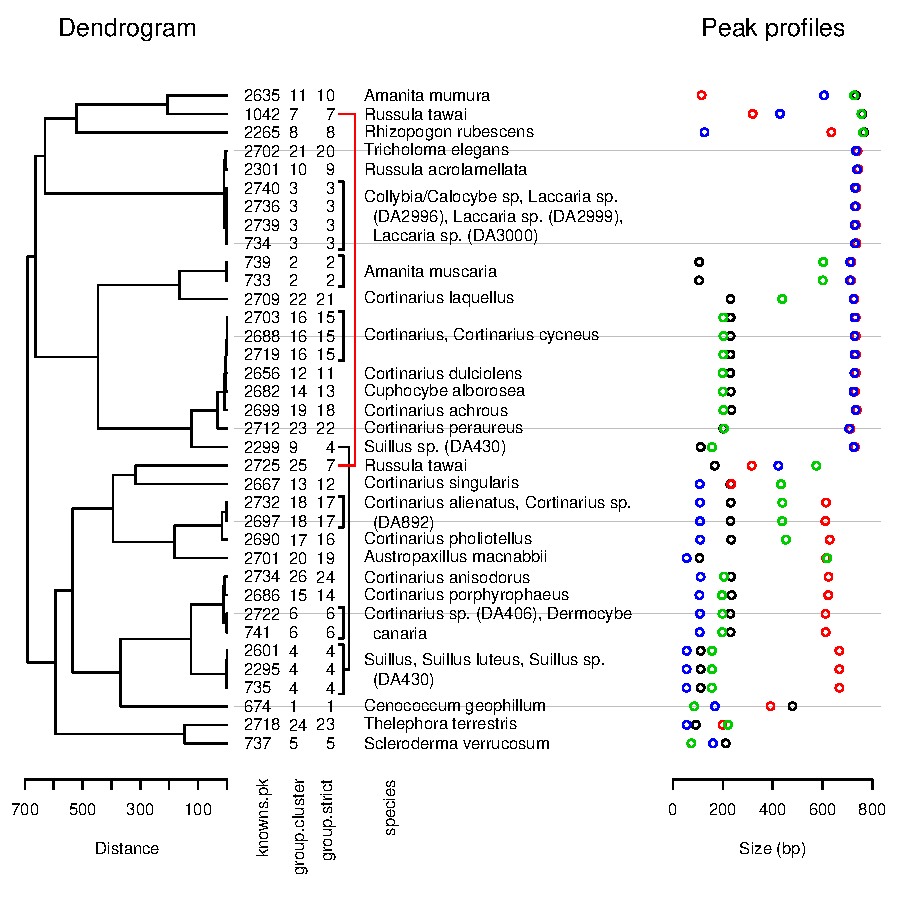
\includegraphics{TRAMPRdemo-012}
\caption{A plot summarising the knowns database \code{demo.knowns}.
  The panels (from left to right) illustrate: (1) the clutering of
  knowns based on TRFLP profile similarity, (2) known names, and group
  indices, and (3) the TRFLP profile for each individual (different
  colours indicate different enzyme/primer combinations).}
\label{fig:knowns}
\end{figure}

\section{Find matches with \code{TRAMP}}

Depending on the size of the samples and knowns databases, and the
speed of your computer, running \code{TRAMP} may be slow.  Optional
arguments to \code{TRAMP} control the strictness of the match
(e.g. number of base pairs difference between sample and knowns
profiles); see the help file \help{TRAMP} for more information.  To
run \code{TRAMP}, run:

\begin{Schunk}
\begin{Sinput}
> fit <- TRAMP(demo.samples, demo.knowns)
\end{Sinput}
\end{Schunk}

A fit may be plotted to inspect the match.  For example, to see the
fit for sample 565, do (See Figure \ref{fig:plot-565} for output):

\begin{Schunk}
\begin{Sinput}
> plot(fit, 565)
\end{Sinput}
\end{Schunk}

\begin{figure}
  \centering
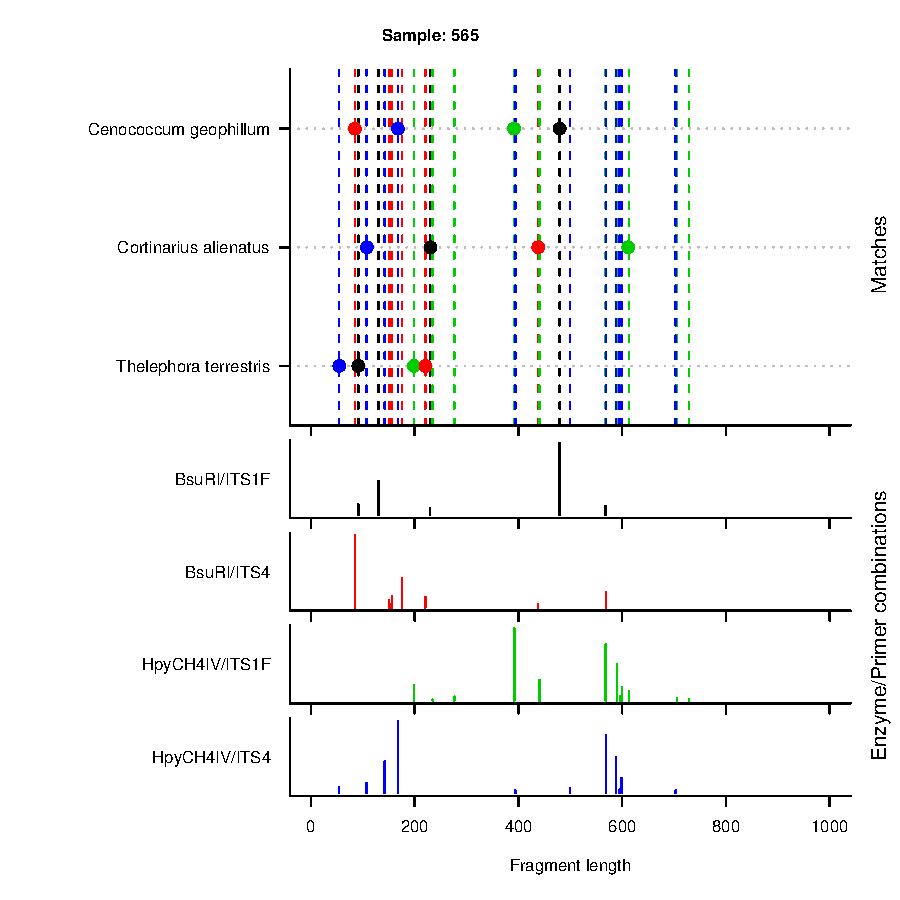
\includegraphics{TRAMPRdemo-015}
\caption{A plot showing the fit of sample 565 against a database of
  knowns.  The sample matches nine knowns, and many unmatched peaks
  remain.  The square points indicate matches between the knowns
  (listed on the \textit{y} axis of the top panel) and the peaks of
  the sample.  The peak profile across four enzyme/primer combinations
  is displayed in the bottom four panels.}
\label{fig:plot-565}
\end{figure}


You can export a PDF containing one fit per page:

\begin{Schunk}
\begin{Sinput}
> pdf("TRAMP_fits.pdf")
> plot(fit)
> dev.off()
\end{Sinput}
\end{Schunk}

The main output of a \code{TRAMP} analysis is a presence/absence
matrix, produced by \code{summary}:

\begin{Schunk}
\begin{Sinput}
> m <- summary(fit)
> m[1:5, 1:5]
\end{Sinput}
\begin{Soutput}
      known
sample   674   733   734   735   737
   101 FALSE FALSE FALSE FALSE FALSE
   102 FALSE FALSE FALSE FALSE FALSE
   110  TRUE FALSE FALSE FALSE FALSE
   111 FALSE FALSE FALSE FALSE FALSE
   117 FALSE FALSE  TRUE FALSE FALSE
\end{Soutput}
\end{Schunk}

\code{TRAMPR} can also use ``unknown knowns''; these are patterns that
repeatedly occur in TRFLP data, but for which a species is currently
unidentified.  The function \code{build.knowns} attempts to spot good
``unknown knowns'' in your data set:

\begin{Schunk}
\begin{Sinput}
> knowns.unk <- build.knowns(demo.samples)
\end{Sinput}
\end{Schunk}

\code{build.knowns} is also useful where your sample data include
profiles from sporocarps.  You can use the argument
\code{restrict=TRUE}, and relax other conditions to generate a knowns
database from only your sporocarps (see the help page
\help{build.knowns}) for more information.  (The command below will
not run on the demonstration data provided, as none of the samples
come from sporocarps.)

\begin{Schunk}
\begin{Sinput}
> knowns.sporocarps <- build.knowns(demo.samples, restrict = TRUE, 
+     min.ratio = 0)
\end{Sinput}
\end{Schunk}

The new knowns database can be added to either the \code{TRAMP} object
or the \code{TRAMPknowns} object.  To add the new knowns to the
\code{TRAMP} object:

\begin{Schunk}
\begin{Sinput}
> fit <- combine(fit, knowns.unk)
\end{Sinput}
\end{Schunk}

Alternatively, to add the new knowns to the \code{TRAMPknowns} object:

\begin{Schunk}
\begin{Sinput}
> demo.knowns <- combine(demo.knowns, knowns.unk)
\end{Sinput}
\end{Schunk}

These are equivalent in their actions on the knowns.  The
\code{knowns} element of \code{fit} and \code{demo.knowns} will be the
same:

\begin{Schunk}
\begin{Sinput}
> identical(demo.knowns, fit$knowns)
\end{Sinput}
\begin{Soutput}
[1] TRUE
\end{Soutput}
\end{Schunk}
%% $ (cheers, emacs!)

The main difference is that if the knowns are added to the
\code{TRAMP} object, then the fit will be rerun automatically.  You
can always extract the modified knowns from a \code{TRAMP} object:

\begin{Schunk}
\begin{Sinput}
> demo.knowns <- fit$knowns
\end{Sinput}
\end{Schunk}
%% $ (cheers, emacs!)

\code{build.knowns} is fairly conservative and may miss some potential
``unknown knowns''.  In particular, ``split peaks'', where the ABI
program identifes two large ``peaks'' occuring within a few base pairs
of each other where only one true peak exists, will often be missed.
You can plot the samples that were not added to the knowns database by
\code{build.knowns} like this:

\begin{Schunk}
\begin{Sinput}
> samples <- setdiff(labels(demo.samples), labels(demo.knowns))
> plot(fit, samples)
\end{Sinput}
\end{Schunk}

Sample 221 shows a clear split peak for BsuRI/ITS1F, and may be a good
potential known:

\begin{Schunk}
\begin{Sinput}
> plot(fit, 221)
\end{Sinput}
\end{Schunk}

or

\begin{Schunk}
\begin{Sinput}
> plot(demo.samples, 221)
\end{Sinput}
\end{Schunk}

will show you the profile (not shown here).  We can add this to the
database using the \code{add.known} function.  As with \code{combine},
this can be used directly on the \code{TRAMP} object or on a knowns
database.  We will use the \code{TRAMP} object again (this generates
a warning, since there are multiple peaks for BsuRI/ITS1F).

\begin{Schunk}
\begin{Sinput}
> fit <- add.known(fit, 221, prompt = FALSE)
\end{Sinput}
\end{Schunk}

Using the \code{summary} function, we can see which samples match this
new known:
\begin{Schunk}
\begin{Sinput}
> names(which(summary(fit)[, "221"]))
\end{Sinput}
\begin{Soutput}
 [1] "221" "224" "310" "311" "339" "579" "580" "583" "585" "586"
\end{Soutput}
\end{Schunk}

Plotting the last of these shows the new known plus two
\textit{Amanita muscaria} knowns (and several other ``unknown knowns''
from running \code{build.knowns}) matching the sample (see Figure
\ref{fig:plot-586}).

\begin{Schunk}
\begin{Sinput}
> plot(fit, 586)
\end{Sinput}
\end{Schunk}

\begin{figure}
  \centering
\includegraphics{TRAMPRdemo-030}
\caption{A plot showing the fit of sample ``586'' against a database
  of knowns, showing the sample matching \textit{Amanita muscaria},
  plus several ``unknown knowns'', including one added manually
  (``Unknown sample: 221'').  In this case, the Unknown sample 221
  appears to be a new \textit{Amanita muscaria}, and this is confirmed
  by grouping (see Figure \ref{fig:plot-586-grouped}).}
\label{fig:plot-586}
\end{figure}

This plot illustrates the need for grouping; since there are multiple
entries for \textit{Amanita muscaria}, it will be counted as a match
twice.  Using \code{grouped=TRUE}, we can group TRFLP profiles that
are very similar or that share species names:

\begin{Schunk}
\begin{Sinput}
> plot(fit, 586, grouped = TRUE)
\end{Sinput}
\end{Schunk}

\begin{figure}
  \centering
\includegraphics{TRAMPRdemo-032}
\caption{A plot showing the fit of sample ``586'' against a database
  of knowns, but with the knowns grouped (compare with Figure
  \ref{fig:plot-586}).  The unknown known has grouped with
  \textit{Amanita muscaria}.  Another group of ``unknown knowns'' also
  matches this sample.
}
\label{fig:plot-586-grouped}
\end{figure}

Output is shown in Figure \ref{fig:plot-586-grouped}; with grouping,
the matches collapse into two separate groups.  Unknown sample 221
groups within the \textit{Amanita muscaria} group.  By allowing
multiple entries for single species, we can keep the error size used
for matching low (there is a discussion of this in the help file
\help{group.knowns}).

The \code{update.TRAMP} function can also interactively add knowns.
See the help file (\help{update.TRAMP}), or just try (output not
shown):

\begin{Schunk}
\begin{Sinput}
> fit <- update(fit)
\end{Sinput}
\end{Schunk}

\section{Using \code{TRAMP} results}

Here we demonstrate a simple principle components analysis of the
community composition of the sample dataset.  [This is not neccesarily
the appropriate analysis type for this kind of data, and we do not
endorse it.]  Once the presence/absence matrix is extracted from the
\code{TRAMP} object, this uses just built-in \R\ functions.  First, we
construct a presence/absence matrix, and restrict this to knowns where
at least one sample matches.  We are using the grouped
presence/absence matrix to include only genuinely different species.

\begin{Schunk}
\begin{Sinput}
> m <- summary(fit, grouped = TRUE)
> m <- m[, colSums(m) > 0]
\end{Sinput}
\end{Schunk}

Next, aggregate the results by soilcore.  Several samples came from
each soil core, and a known is scored as being present if it is
present in \code{any} of the samples.  This produces a much smaller
matrix (see output in Figure \ref{fig:presence-absence-matrix}).

\begin{Schunk}
\begin{Sinput}
> cores <- fit$samples$info$soilcore.fk
> m.bycore <- aggregate(m, by = list(cores = cores), any)
> rownames(m.bycore) <- m.bycore$cores
> m.bycore <- m.bycore[-1]
> m.bycore
\end{Sinput}
\end{Schunk}

(The \code{m.bycore[-1]} line removes an index column that
\code{aggregate} creates).

\begin{figure}
\begin{Schunk}
\begin{Soutput}
       1     2     3     4     5     6     7     8     9    10    11    19
2  FALSE FALSE FALSE FALSE FALSE FALSE FALSE FALSE FALSE  TRUE FALSE FALSE
3  FALSE FALSE FALSE FALSE FALSE FALSE FALSE FALSE  TRUE FALSE FALSE FALSE
4  FALSE FALSE FALSE FALSE FALSE FALSE FALSE FALSE  TRUE  TRUE FALSE FALSE
5   TRUE FALSE FALSE FALSE FALSE  TRUE FALSE FALSE FALSE  TRUE FALSE FALSE
6   TRUE FALSE FALSE FALSE FALSE  TRUE FALSE FALSE  TRUE  TRUE FALSE  TRUE
12 FALSE FALSE FALSE  TRUE FALSE FALSE FALSE FALSE FALSE FALSE FALSE FALSE
13 FALSE FALSE FALSE FALSE FALSE FALSE  TRUE FALSE FALSE FALSE FALSE FALSE
14 FALSE FALSE FALSE FALSE  TRUE FALSE  TRUE FALSE FALSE FALSE FALSE FALSE
15 FALSE FALSE FALSE  TRUE FALSE FALSE FALSE FALSE FALSE FALSE FALSE FALSE
16 FALSE FALSE FALSE  TRUE  TRUE FALSE  TRUE FALSE FALSE FALSE FALSE FALSE
17 FALSE FALSE FALSE FALSE FALSE  TRUE FALSE FALSE  TRUE  TRUE  TRUE FALSE
18  TRUE FALSE FALSE FALSE FALSE  TRUE FALSE FALSE FALSE FALSE FALSE FALSE
19 FALSE FALSE FALSE FALSE FALSE FALSE FALSE FALSE FALSE  TRUE FALSE FALSE
20 FALSE FALSE FALSE FALSE FALSE FALSE FALSE FALSE FALSE  TRUE FALSE FALSE
21 FALSE  TRUE FALSE FALSE FALSE FALSE FALSE FALSE FALSE FALSE FALSE FALSE
32 FALSE FALSE FALSE FALSE  TRUE FALSE  TRUE  TRUE FALSE FALSE FALSE FALSE
33 FALSE FALSE  TRUE FALSE FALSE FALSE  TRUE FALSE FALSE FALSE FALSE FALSE
34 FALSE FALSE FALSE FALSE FALSE FALSE FALSE FALSE FALSE FALSE FALSE FALSE
35 FALSE FALSE FALSE FALSE  TRUE FALSE FALSE FALSE FALSE FALSE FALSE FALSE
36 FALSE FALSE FALSE FALSE FALSE FALSE  TRUE FALSE FALSE FALSE FALSE FALSE
      20    22    23    24    28    29
2  FALSE FALSE  TRUE FALSE FALSE  TRUE
3  FALSE FALSE FALSE  TRUE FALSE FALSE
4  FALSE FALSE FALSE FALSE FALSE FALSE
5   TRUE FALSE FALSE FALSE FALSE FALSE
6  FALSE  TRUE FALSE FALSE FALSE FALSE
12 FALSE FALSE FALSE FALSE FALSE FALSE
13 FALSE FALSE FALSE FALSE FALSE FALSE
14 FALSE FALSE FALSE FALSE FALSE FALSE
15 FALSE FALSE FALSE FALSE FALSE FALSE
16 FALSE FALSE FALSE FALSE FALSE FALSE
17 FALSE  TRUE FALSE FALSE FALSE FALSE
18 FALSE  TRUE FALSE FALSE FALSE FALSE
19 FALSE FALSE FALSE FALSE FALSE FALSE
20 FALSE  TRUE FALSE FALSE  TRUE FALSE
21 FALSE FALSE FALSE FALSE FALSE FALSE
32 FALSE FALSE FALSE FALSE FALSE FALSE
33 FALSE FALSE FALSE FALSE FALSE FALSE
34 FALSE FALSE FALSE FALSE FALSE FALSE
35 FALSE FALSE FALSE FALSE FALSE FALSE
36 FALSE FALSE FALSE FALSE FALSE FALSE
\end{Soutput}
\end{Schunk}
\caption{Presence/absence matrix for the soil core data.  Rows
  represent different soil cores, with row names corresponding to
  \code{soilcore.pk} values in the \code{soilcore} table.  Columns
  correspond to groups of knowns, each of which may represent multiple
  knowns entries.}
\label{fig:presence-absence-matrix}
\end{figure}

Now, determine which vegetation type applies to each row in the
presence/absence matrix.
\begin{Schunk}
\begin{Sinput}
> core.veg <- soilcore$vegetation[match(rownames(m.bycore), soilcore$soilcore.pk)]
\end{Sinput}
\end{Schunk}

Next, create a rank-abundance diagram of the data (see Figure
\ref{fig:rankabundance} for output).

\begin{Schunk}
\begin{Sinput}
> sp.freq <- sort(colSums(m.bycore), decreasing = TRUE)
> plot(sp.freq, xlab = "Species rank", ylab = "Species frequency", 
+     type = "o", pch = 19)
\end{Sinput}
\end{Schunk}

You can also calculate mean species richness across the different
vegetation types:
\begin{Schunk}
\begin{Sinput}
> tapply(rowSums(m.bycore), core.veg, mean)
\end{Sinput}
\begin{Soutput}
Nothofagus solandri      Pinus contorta 
                3.0                 1.5 
\end{Soutput}
\end{Schunk}

\begin{figure}
  \centering
\includegraphics{TRAMPRdemo-040}
\caption{Rank-abundance diagram for 18 species
  present across 20 soilcores.
}
\label{fig:rankabundance}
\end{figure}

Finally, run a principle components analysis, and create a plot of the
first two principle axes.  To distinguish between the two different
forest types, we determine the vegetation type for each core, and
create a vector of colours so that cores from \textit{Nothofagus
  solandri} stands are blue circles and cores from \textit{Pinus
  contorta} stands are red crosses (see Figure \ref{fig:pca} for
output).

\begin{Schunk}
\begin{Sinput}
> pca <- prcomp(m.bycore)
> col <- c("blue", "red")[as.integer(core.veg)]
> pch <- c(1, 3)[as.integer(core.veg)]
> plot(pca$x[, 1], pca$x[, 2], col = col, pch = pch, xlab = "PC1", 
+     ylab = "PC2")
> legend("top", levels(core.veg), col = c("blue", "red"), pch = c(1, 
+     3))
\end{Sinput}
\end{Schunk}

\begin{figure}
  \centering
\includegraphics{TRAMPRdemo-042}
\caption{Principle components analysis of soil community data.
  Different points represent different soil cores, and colours
  distinguish forest types.  [We are not endorsing PCA as an
  appropriate analysis for these data.]
}
\label{fig:pca}
\end{figure}

\section{Managing and saving knowns}
\label{sec:knowns-manage}

We can save the modified knowns database in two ways.  If you want to
edit any aspect of the knowns (e.g. species names), or update an
external database, use \code{write.TRAMPknowns}:

\begin{Schunk}
\begin{Sinput}
> write.TRAMPknowns(fit$knowns, "my_knowns")
\end{Sinput}
\end{Schunk}
%% $

This will create files \code{my\_knowns\_info.csv}  and
\code{my\_knowns\_data.csv}, which contain the information required to
build the knowns.  The files are documented in
\help{write.TRAMPknowns}, and can be edited in Excel\footnote{If
  editing in Excel, when saving it will warn you about losing
  information when saving as a csv file -- ignore these warnings, as
  \code{TRAMP} requires that the data are saved as csv.}.  The knowns
can be reloaded in a future \R\ session by:

\begin{Schunk}
\begin{Sinput}
> my.knowns <- read.TRAMPknowns("my_knowns")
\end{Sinput}
\end{Schunk}

Alternatively, knowns can be saved like any other \R\ object, using
\code{save} and \code{load}.  To save your knowns, do:

\begin{Schunk}
\begin{Sinput}
> my.knowns <- fit$knowns
> save(my.knowns, file = "my_knowns.Rdata")
\end{Sinput}
\end{Schunk}
%% $

This will create a single file \code{my\_knowns.Rdata}, which is a
non-human readable Rdata file containing the knowns object.  Note that
the object saved must be an object named in the global environment, so
we must extract the knowns first.

To reload
this in a future \R\ session, do:
\begin{Schunk}
\begin{Sinput}
> load("my_knowns.Rdata")
\end{Sinput}
\end{Schunk}

This will create an object called \code{my.knowns} in the global
environment.

\section{Concluding remarks}
This is a brief introduction, but which should cover most of the
functionality of the \code{TRAMPR} package.  Detailed information can
be found in the reference manual; type \code{library(help=TRAMPR)} for
a list of topics.  In particular, the behaviour of most functions can
be altered by changing optional arguments.

\end{document}
